%% Per aspera ad astra.
% !TeX spellcheck = pl_PL
%%%%%%%%%%%%%%%%%%%%%%%%%%%%%%%%%%%%%%%%%%%
%                                        %
% Szablon pracy dyplomowej inzynierskiej %
% zgodny  z aktualnymi  przepisami  SZJK %
%                                        %
%%%%%%%%%%%%%%%%%%%%%%%%%%%%%%%%%%%%%%%%%%
%                                        %
%  (c) Krzysztof Simiński, 2018-2023     %
%                                        %
%%%%%%%%%%%%%%%%%%%%%%%%%%%%%%%%%%%%%%%%%%
%                                        %
% Najnowsza wersja szablonów jest        %
% podstępna pod adresem                  %
% github.com/ksiminski/polsl-aei-theses  %
%                                        %
%%%%%%%%%%%%%%%%%%%%%%%%%%%%%%%%%%%%%%%%%%
%
% Projekt LaTeXowy zapewnia odpowiednie formatowanie pracy,
% zgodnie z wymaganiami Systemu zapewniania jakości kształcenia.
% Proszę nie zmieniać ustawień formatowania (np. fontu,
% marginesów, wytłuszczeń, kursywy itd. ).
%
% Projekt można kompilować na kilka sposobów.
%
% 1. kompilacja pdfLaTeX
%
% pdflatex main
% bibtex   main
% pdflatex main
% pdflatex main
%
% 2. kompilacja XeLaTeX
%
% Kompilatacja przy użyciu XeLaTeXa różni się tym, że na stronie
% tytułowej używany jest font Calibri. Wymaga to jego uprzedniego
% zainstalowania.
%
% xelatex main
% bibtex  main
% xelatex main
% xelatex main
%
%%%%%%%%%%%%%%%%%%%%%%%%%%%%%%%%%%%%%%%%%%%%%%%%%%%%%
% W przypadku pytań, uwag, proszę pisać na adres:   %
%      krzysztof.siminski(małpa)polsl.pl            %
%%%%%%%%%%%%%%%%%%%%%%%%%%%%%%%%%%%%%%%%%%%%%%%%%%%%%
%
% Chcemy ulepszać szablony LaTeXowe prac dyplomowych.
% Wypełniając ankietę spod poniższego adresu pomogą
% Państwo nam to zrobić. Ankieta jest całkowicie
% anonimowa. Dziękujemy!

% https://docs.google.com/forms/d/e/1FAIpQLScyllVxNKzKFHfILDfdbwC-jvT8YL0RSTFs-s27UGw9CKn-fQ/viewform?usp=sf_link
%
%%%%%%%%%%%%%%%%%%%%%%%%%%%%%%%%%%%%%%%%%%%%%%%%%%%%%%%%%%%%%%%%%%%%%%%%%

% Autor pracy inżynierskiej na bazie szablonu,
% oraz wszelkich poprawek:
% Daniel Chydziński

%%%%%%%%%%%%%%%%%%%%%%%%%%%%%%%%%%%%%%%%%%%%%%%
%                                             %
% PERSONALIZACJA PRACY – DANE PRACY           %
%                                             %
%%%%%%%%%%%%%%%%%%%%%%%%%%%%%%%%%%%%%%%%%%%%%%%

% Proszę wpisać swoje dane w poniższych definicjach.

% TODO
% dane autora
\newcommand{\FirstNameAuthor}{Daniel}
\newcommand{\SurnameAuthor}{Chydziński}
\newcommand{\IdAuthor}{296781}

% drugi autor:
%\newcommand{\FirstNameCoauthor}{Imię}   % Jeżeli jest drugi autor, to tutaj należy podać imię.
%\newcommand{\SurnameCoauthor}{Nazwisko} % Jeżeli jest drugi autor, to tutaj należy podać nazwisko.
%\newcommand{\IdCoauthor}{$\langle$wpisać właściwy$\rangle$}  % numer albumu drugiego autora (bez $\langle$ i $\rangle$)
% Gdy nie ma drugiego autora, należy zostawić poniższe definicje puste, jak poniżej. Gdy jest drugi autor, należy zakomentować te linie.
\newcommand{\FirstNameCoauthor}{} % Jeżeli praca ma tylko jednego autora, to dane drugiego autora zostają puste.
\newcommand{\SurnameCoauthor}{}   % Jeżeli praca ma tylko jednego autora, to dane drugiego autora zostają puste.
\newcommand{\IdCoauthor}{}  % Jeżeli praca ma tylko jednego autora, to dane drugiego autora zostają puste.
%%%%%%%%%%

\newcommand{\Supervisor}{dr Aleksander Staszulonek}     % dane promotora (bez $\langle$ i $\rangle$)
\newcommand{\Title}{Analiza błędów pomiaru położenia platformy mobilnej}           % tytuł pracy po polsku
\newcommand{\TitleAlt}{Mobile platform position errors analysis}                     % thesis title in English
\newcommand{\Program}{Automatyka i Robotyka}            % kierunek studiów  (bez $\langle$ i $\rangle$)
\newcommand{\Specialisation}{Automatyka Procesowa}     % specjalność  (bez $\langle$ i $\rangle$)
\newcommand{\Departament}{Automatyki i Robotyki}        % katedra promotora  (bez $\langle$ i $\rangle$)

% Jeżeli został wyznaczony promotor pomocniczy lub opiekun, proszę go/ją wpisać ...
\newcommand{\Consultant}{$\langle$stopień naukowy imię i nazwisko$\rangle$} % dane promotora pomocniczego, opiekuna (bez $\langle$ i $\rangle$)
% ... w przeciwnym razie proszę zostawić puste miejsce jak poniżej:
%\newcommand{\Consultant}{} % brak promotowa pomocniczego / opiekuna

% koniec fragmentu do modyfikacji
%%%%%%%%%%%%%%%%%%%%%%%%%%%%%%%%%%%%%%%%%%

%%%%%%%%%%%%%%%%%%%%%%%%%%%%%%%%%%%%%%%%%%%%%%%
%                                             %
% KONIEC PERSONALIZACJI PRACY                 %
%                                             %
%%%%%%%%%%%%%%%%%%%%%%%%%%%%%%%%%%%%%%%%%%%%%%%

%%%%%%%%%%%%%%%%%%%%%%%%%%%%%%%%%%%%%%%%%%%%%%%
%                                             %
% PROSZĘ NIE MODYFIKOWAĆ PONIŻSZYCH USTAWIEŃ! %
%                                             %
%%%%%%%%%%%%%%%%%%%%%%%%%%%%%%%%%%%%%%%%%%%%%%%

\documentclass[a4paper,twoside,12pt]{book}
\usepackage[utf8]{inputenc}                                      
\usepackage[T1]{fontenc}  
\usepackage{amsmath,amsfonts,amssymb,amsthm}
\usepackage[british,polish]{babel} 
\usepackage{indentfirst}
\usepackage{xurl}
\usepackage{xstring}
\usepackage{ifthen}



\usepackage{ifxetex}

\ifxetex
	\usepackage{fontspec}
	\defaultfontfeatures{Mapping=tex—text} % to support TeX conventions like ``——-''
	\usepackage{xunicode} % Unicode support for LaTeX character names (accents, European chars, etc)
	\usepackage{xltxtra} % Extra customizations for XeLaTeX
\else
	\usepackage{lmodern}
\fi



\usepackage[margin=2.5cm]{geometry}
\usepackage{graphicx} 
\usepackage{hyperref}
\usepackage{booktabs}
\usepackage{tikz}
\usepackage{pgfplots}
\usepackage{mathtools}
\usepackage{geometry}
\usepackage{subfig}   % subfigures
\usepackage[page]{appendix} % toc,
\renewcommand{\appendixtocname}{Dodatki}
\renewcommand{\appendixpagename}{Dodatki}
\renewcommand{\appendixname}{Dodatek}

\usepackage{csquotes}
\usepackage[natbib=true,backend=bibtex,maxbibnames=99]{biblatex}  % kompilacja bibliografii BibTeXem
%\usepackage[natbib=true,backend=biber,maxbibnames=99]{biblatex}  % kompilacja bibliografii Biberem
\bibliography{biblio}

\usepackage{ifmtarg}   % empty commands  

\usepackage{setspace}
\onehalfspacing


\frenchspacing

%%%%%%%%%%%%%%%%%%%%%%%%%%%%%%%%%%
% środowiska dla definicji, twierdzenia, przykładu
\usepackage{amsthm}

\newtheorem{Definition}{Definicja}
\newtheorem{Example}{Przykład}
\newtheorem{Theorem}{Twierdzenie}
%%%%%%%%%%%%%%%%%%%%%%%%%%%%%%%%%%

%%%% TODO LIST GENERATOR %%%%%%%%%

\usepackage{color}
\definecolor{brickred}      {cmyk}{0   , 0.89, 0.94, 0.28}

\makeatletter \newcommand \kslistofremarks{\section*{Uwagi} \@starttoc{rks}}
  \newcommand\l@uwagas[2]
    {\par\noindent \textbf{#2:} %\parbox{10cm}
{#1}\par} \makeatother


\newcommand{\ksremark}[1]{%
{%\marginpar{\textdbend}
{\color{brickred}{[#1]}}}%
\addcontentsline{rks}{uwagas}{\protect{#1}}%
}

\newcommand{\comma}{\ksremark{przecinek}}
\newcommand{\nocomma}{\ksremark{bez przecinka}}
\newcommand{\styl}{\ksremark{styl}}
\newcommand{\ortografia}{\ksremark{ortografia}}
\newcommand{\fleksja}{\ksremark{fleksja}}
\newcommand{\pauza}{\ksremark{pauza `--', nie dywiz `-'}}
\newcommand{\kolokwializm}{\ksremark{kolokwializm}}
\newcommand{\cudzyslowy}{\ksremark{,,polskie cudzysłowy''}}

%%%%%%%%%%%%%% END OF TODO LIST GENERATOR %%%%%%%%%%%

\newcommand{\printCoauthor}{%		
    \StrLen{\FirstNameCoauthor}[\FNCoALen]
    \ifthenelse{\FNCoALen > 0}%
    {%
		{\large\bfseries\Coauthor\par}
	
		{\normalsize\bfseries \LeftId: \IdCoauthor\par}
    }%
    {}
} 

%%%%%%%%%%%%%%%%%%%%%
\newcommand{\autor}{%		
    \StrLen{\FirstNameCoauthor}[\FNCoALenXX]
    \ifthenelse{\FNCoALenXX > 0}%
    {\FirstNameAuthor\ \SurnameAuthor, \FirstNameCoauthor\ \SurnameCoauthor}%
	{\FirstNameAuthor\ \SurnameAuthor}%
}
%%%%%%%%%%%%%%%%%%%%%

\StrLen{\FirstNameCoauthor}[\FNCoALen]
\ifthenelse{\FNCoALen > 0}%
{%
\author{\FirstNameAuthor\ \SurnameAuthor, \FirstNameCoauthor\ \SurnameCoauthor}
}%
{%
\author{\FirstNameAuthor\ \SurnameAuthor}
}%

%%%%%%%%%%%% ZYWA PAGINA %%%%%%%%%%%%%%%
% brak kapitalizacji zywej paginy
\usepackage{fancyhdr}
\pagestyle{fancy}
\fancyhf{}
\fancyhead[LO]{\nouppercase{\it\rightmark}}
\fancyhead[RE]{\nouppercase{\it\leftmark}}
\fancyhead[LE,RO]{\it\thepage}


\fancypagestyle{tylkoNumeryStron}{%
   \fancyhf{} 
   \fancyhead[LE,RO]{\it\thepage}
}

\fancypagestyle{bezNumeracji}{%
   \fancyhf{} 
   \fancyhead[LE,RO]{}
}


\fancypagestyle{NumeryStronNazwyRozdzialow}{%
   \fancyhf{} 
   \fancyhead[LE]{\nouppercase{\autor}}
   \fancyhead[RO]{\nouppercase{\leftmark}} 
   \fancyfoot[CE, CO]{\thepage}
}


%%%%%%%%%%%%% OBCE WTRETY  
\newcommand{\obcy}[1]{\emph{#1}}
\newcommand{\english}[1]{{\selectlanguage{british}\obcy{#1}}}
%%%%%%%%%%%%%%%%%%%%%%%%%%%%%

% polskie oznaczenia funkcji matematycznych
\renewcommand{\tan}{\operatorname {tg}}
\renewcommand{\log}{\operatorname {lg}}

% jeszcze jakies drobiazgi

\newcounter{stronyPozaNumeracja}

%%%%%%%%%%%%%%%%%%%%%%%%%%% 
\newcommand{\printOpiekun}[1]{%		

    \StrLen{\Consultant}[\mystringlen]
    \ifthenelse{\mystringlen > 0}%
    {%
       {\large{\bfseries OPIEKUN, PROMOTOR POMOCNICZY}\par}
       
       {\large{\bfseries \Consultant}\par}
    }%
    {}
} 
%
%%%%%%%%%%%%%%%%%%%%%%%%%%%%%%%%%%%%%%%%%%%%%%
 
% Proszę nie modyfikować poniższych definicji!
\newcommand{\Author}{\FirstNameAuthor\ \MakeUppercase{\SurnameAuthor}} 
\newcommand{\Coauthor}{\FirstNameCoauthor\ \MakeUppercase{\SurnameCoauthor}}
\newcommand{\Type}{PROJEKT INŻYNIERSKI}
\newcommand{\Faculty}{Wydział Automatyki, Elektroniki i Informatyki} 
\newcommand{\Polsl}{Politechnika Śląska}
\newcommand{\Logo}{politechnika_sl_logo_bw_pion_pl.pdf}
\newcommand{\LeftId}{Nr albumu}
\newcommand{\LeftProgram}{Kierunek}
\newcommand{\LeftSpecialisation}{Specjalność}
\newcommand{\LeftSUPERVISOR}{PROWADZĄCY PRACĘ}
\newcommand{\LeftDEPARTMENT}{KATEDRA}
%%%%%%%%%%%%%%%%%%%%%%%%%%%%%%%%%%%%%%%%%%%%%%

%%%%%%%%%%%%%%%%%%%%%%%%%%%%%%%%%%%%%%%%%%%%%%%
%                                             %
% KONIEC USTAWIEŃ                             %
%                                             %
%%%%%%%%%%%%%%%%%%%%%%%%%%%%%%%%%%%%%%%%%%%%%%%

%%%%%%%%%%%%%%%%%%%%%%%%%%%%%%%%%%%%%%%%%%%%%%%
%                                             %
% MOJE PAKIETY, USTAWIENIA ITD                %
%                                             %
%%%%%%%%%%%%%%%%%%%%%%%%%%%%%%%%%%%%%%%%%%%%%%%

% Tutaj proszę umieszczać swoje pakiety, makra, ustawienia itd.


 
%%%%%%%%%%%%%%%%%%%%%%%%%%%%%%%%%%%%%%%%%%%%%%%%%%%%%%%%%%%%%%%%%%%%%
% listingi i fragmentu kodu źródłowego 
% pakiet: listings lub minted
% % % % % % % % % % % % % % % % % % % % % % % % % % % % % % % % % % % 

% biblioteka listings
\usepackage{listings}
\lstset{%
morekeywords={string,exception,std,vector},% słowa kluczowe rozpoznawane przez pakiet listings
language=C++,% C, Matlab, Python, SQL, TeX, XML, bash, ... – vide https://www.ctan.org/pkg/listings
commentstyle=\textit,%
identifierstyle=\textsf,%
keywordstyle=\sffamily\bfseries, %\texttt, %
%captionpos=b,%
tabsize=3,%
frame=lines,%
numbers=left,%
numberstyle=\tiny,%
numbersep=5pt,%
breaklines=true,%
escapeinside={@*}{*@},%
}

\usepackage{enumerate}

% % % % % % % % % % % % % % % % % % % % % % % % % % % % % % % % % % % 
% pakiet minted
%\usepackage{minted}

% pakiet wymaga specjalnego kompilowania:
% pdflatex -shell-escape main.tex
% xelatex  -shell-escape main.tex

%\usepackage[chapter]{minted} % [section]
%%\usemintedstyle{bw}   % czarno-białe kody 
%
%\setminted % https://ctan.org/pkg/minted
%{
%%fontsize=\normalsize,%\footnotesize,
%%captionpos=b,%
%tabsize=3,%
%frame=lines,%
%framesep=2mm,
%numbers=left,%
%numbersep=5pt,%
%breaklines=true,%
%escapeinside=@@,%
%}

%%%%%%%%%%%%%%%%%%%%%%%%%%%%%%%%%%%%%%%%%%%%%%%%%%%%%%%%%%%%%%%%%%%%%

%%%%%%%%%%%%%%%%%%%%%%%%%%%%%%%%%%%%%%%%%%%%%%%
%                                             %
% KONIEC MOICH USTAWIEŃ                       %
%                                             %
%%%%%%%%%%%%%%%%%%%%%%%%%%%%%%%%%%%%%%%%%%%%%%%

\begin{document}
%\kslistofremarks

\frontmatter

%%%%%%%%%%%%%%%%%%%%%%%%%%%%%%%%%%%%%%%%%%%%%%%
%                                             %
% PROSZĘ NIE MODYFIKOWAĆ STRONY TYTUŁOWEJ!    %
%                                             %
%%%%%%%%%%%%%%%%%%%%%%%%%%%%%%%%%%%%%%%%%%%%%%%

\pagestyle{empty}
{
	\newgeometry{top=1.5cm,%
	             bottom=2.5cm,%
	             left=3cm,
	             right=2.5cm}
 
	\ifxetex 
	  \begingroup
	  \setsansfont{Calibri}
	   
	\fi 
	 \sffamily
	\begin{center}
	\includegraphics[width=100mm]{\Logo}
	 
	
	{\Large\bfseries\Type\par}
	
	\vfill  \vfill  
			 
	{\large\Title\par}
	
	\vfill  
		
	{\large\bfseries\Author\par}
	
	{\normalsize\bfseries \LeftId: \IdAuthor}

	\printCoauthor
	
	\vfill  		
 
	{\large{\bfseries \LeftProgram:} \Program\par} 
	
	{\large{\bfseries \LeftSpecialisation:} \Specialisation\par} 
	 		
	\vfill  \vfill 	\vfill 	\vfill 	\vfill 	\vfill 	\vfill  
	 
	{\large{\bfseries \LeftSUPERVISOR}\par}
	
	{\large{\bfseries \Supervisor}\par}
				
	{\large{\bfseries \LeftDEPARTMENT\ \Departament} \par}
		
	{\large{\bfseries \Faculty}\par}
		
	\vfill  \vfill  

    
	\vfill  \vfill  
		
    {\large\bfseries  Gliwice \the\year}

   \end{center}	
       \ifxetex 
       	  \endgroup
       \fi
	\restoregeometry
}
  
%%%%%%%%%%%%%%%%%%%%%%%%%%%%%%%%%%%%%%%%%%%%%%%
%                                             %
% KONIEC STRONY TYTUŁOWEJ                     %
%                                             %
%%%%%%%%%%%%%%%%%%%%%%%%%%%%%%%%%%%%%%%%%%%%%%%  

\cleardoublepage

\rmfamily\normalfont
\pagestyle{empty}

%%% tu można pisać

\subsubsection*{Tytuł pracy} 
\Title

\subsubsection*{Streszczenie}  
(Streszczenie pracy – odpowiednie pole w systemie APD powinno zawierać kopię tego streszczenia.)

\subsubsection*{Słowa kluczowe} 
(2-5 slow (fraz) kluczowych, oddzielonych przecinkami)

\subsubsection*{Thesis title} 
\begin{otherlanguage}{british}
\TitleAlt
\end{otherlanguage}

\subsubsection*{Abstract} 
\begin{otherlanguage}{british}
(Thesis abstract – to be copied into an appropriate field during an electronic submission – in English.)
\end{otherlanguage}
\subsubsection*{Key words}  
\begin{otherlanguage}{british}
(2-5 keywords, separated by commas)
\end{otherlanguage}

%%%%%%%%%%%%%%%%%% SPIS TRESCI %%%%%%%%%%%%%%%%%%%%%%
% Add \thispagestyle{empty} to the toc file (main.toc), because \pagestyle{empty} doesn't work if the TOC has multiple pages
\addtocontents{toc}{\protect\thispagestyle{empty}}
\tableofcontents

%%%%%%%%%%%%%%%%%%%%%%%%%%%%%%%%%%%%%%%%%%%%%%%%%%%%%
\setcounter{stronyPozaNumeracja}{\value{page}}
\mainmatter
\pagestyle{empty}

\cleardoublepage

\pagestyle{NumeryStronNazwyRozdzialow}

%%%%%%%%%%%%%% wlasciwa tresc pracy %%%%%%%%%%%%%%%%%

%%%%%%%%%%%%%% rozdział 1 - wstęp %%%%%%%%%%%%%%%%%
\chapter{Wstęp}
\label{ch:wstep}

Robotyka to obszar badawczy i~techniczny poświęcony teorii, konstrukcji oraz praktycznym zastosowaniom robotów. Elementami wykonawczymi układów zrobotyzowanych są najczęściej silniki lub siłowniki, te drugie nierzadko napędzane wewnętrznie silnikami. Rodzajem maszyny zamieniającej jeden rodzaj energii --- w~robotyce najczęściej elektryczną --- na energię mechaniczną, czego celem jest wprawienie w~ruch elementów ruchomych.

W przypadku prostych układów (Definicja~\ref{def:uklad}), takich jak podajnik taśmowy napędzany pojedynczym silnikiem, dokładność (Definicja~\ref{def:dokladnosc}) sterowania nie ma wysokiego priorytetu. Najważniejsze jest, by element znajdujący się na taśmie przejechał z~punktu A~do punktu B~z~pewną prędkością, a~jego położeniem zajmą się inne czujniki. Jednak gdy silnik napędza ramię robota, pojazd lub drona, ważne jest, by utrzymywał stałą prędkość i/lub wykonywał określoną ilość obrotów.

\begin{Definition}[Układ sterowania]\label{def:uklad}
   Układ służący do kontroli pożądanego urządzenia przy pomocy wybranego zasobu narzędzi, w~tym zamkniętej pętli z~ujemnym sprzężeniem zwrotnym (Definicja~\ref{def:petla}).
\end{Definition}

\begin{Definition}[Pętla]\label{def:petla}
    Typ struktury układu umożliwiający mu reakcję na informację zwrotną o~jego stanie (sprzężenie zwrotne) pochodzącą z czujników.
\end{Definition}

\begin{Definition}[Dokładność]\label{def:dokladnosc}
    Stopień zgodności pomiędzy rzeczywistymi wartościami a~wartościami określonymi lub mierzonymi.
\end{Definition}

Z tego powodu, jednym z~wyzwań, z~jakimi mierzyli się pionierzy automatycy-robotycy jest dokładne sterowanie tworzonymi przez siebie układami. Jest to kwestia o~tyle istotna, że gdy odpowiedź układu odbiega --- nawet w niewielkim stopniu --- od wartości zadanej, staje się on znacząco trudniejszy w~użytkowaniu (sterowaniu), a w skrajnych przypadkach bezużyteczny. W~przypadku ramienia robota, brak dokładności sterowania doprowadzi układ do osiągnięcia innej lokalizacji niż pożądana. W~przypadku drona, prawdopodobnie całkowicie uniemożliwi lot z~powodu nierówności sił nośnych. Zaś w~przypadku pojazdów autonomicznych, przejechanie odległości innej niż zadana przez operatora. Jako rozwiązanie tego problemu, powstał poddział robotyki zwany odometrią (Definicja~\ref{def:odometria}). 

\begin{Definition}[Odometria]\label{def:odometria}
    Dział nauk technicznych na pograniczu robotyki i~miernictwa, zajmujący się użyciem różnego rodzaju czujników w~celu oszacowania położenia ruchomego układu względem pozycji startowej w przestrzeni fizycznej.
\end{Definition}

Współcześni automatycy-robotycy będący na początku swojej ścieżki edukacji/kariery, lub zajmujący się robotyką jedynie hobbystycznie, również mierzą się prędzej czy później z~problemem dokładności sterowania układu. W~obecnych czasach istnieje wiele sposobów rozwiązania go.

Celem niniejszej pracy inżynierskiej jest zaprojektowanie i~wykonanie fizycznego modelu platformy mobilnej (zwanej dalej pojazdem) oraz aplikacji do jej kontroli. Następnie zastosowanie i~przetestowanie eksperymentalne wybranej metody zwiększenia dokładności układu z~użyciem ujemnego sprzężenia zwrotnego. Na końcu otrzymane wyniki zostaną przeanalizowane pod kątem użyteczności i skuteczności wybranej metody w warunkach rzeczywistych.

Praca podzielona została na następujące rozdziały\cite{bib:wymaganiapracy}:
\begin{enumerate}
    \item Wstęp --- wprowadzenie do tematu, krótkie omówienie istoty problemu, zakres pracy, opis rozdziałów.
    \item Analiza tematu --- omówienie tematu w kontekście aktualnego stanu wiedzy o poruszanym problemie (ang. \english{state of art}), oraz szczegółowe jego sformułowanie.
    \item Założenia i narzędzia --- opis wymagań postawionych przy tworzeniu projektu wraz z uzasadnieniem wyboru, a także lista użytych narzędzi.
    \item Projekt i wykonanie --- szczegółowe omówienie sposobu wykonania modelu pojazdu, układu elektronicznego, aplikacji, kodu mikroprocesora i narzędzi pobocznych. Każdemu elementowi odpowiada podrozdział.
    \item Weryfikacja i walidacja --- zastosowane metody badawcze i wykonane eksperymenty, oraz napotkane i usunięte błędy.
    \item Podsumowanie i wnioski --- skomentowanie uzyskanych wyników pod kątem osiągnięcia założonych celów, analiza i dalsze kroki.
\end{enumerate}

%%%%%%%%%%%%%% rozdział 2 - analiza %%%%%%%%%%%%%%%%%
\chapter{[Analiza tematu]}
\section{Detekcja położenia wału silnika}
\label{ch:analizaenkodery}

Problem synchronizowania silników elektrycznych znany jest w~dziedzinie automatyki od dziesiątek lat. Początki badania silników sięgają XIX wieku, kiedy to Michael Faraday oraz inni naukowcy eksperymentowali ze wykorzystaniem elektromagnetyzmu\cite{bib:pierwszesilniki}. Pierwsze silniki elektryczne były prymitywne i~nie miały zaawansowanych metod sterowania. Wczesne próby pozycjonowania opierały się głównie na prostych mechanizmach, takich jak przekładnie i~sprzęgła.

W miarę postępu technologicznego, szczególnie w~XX wieku, rozwijano bardziej zaawansowane metody pozycjonowania. Pojawiły się pierwsze systemy sterowania, wykorzystujące technologię zwrotną informacji, mającą na celu monitorowanie i~regulację położenia wałów silników. Jednak precyzja tych rozwiązań była ograniczona, a~dokładność pozycjonowania nie zawsze spełniała wymagania coraz bardziej zaawansowanych zastosowań.

Dopiero wprowadzenie enkoderów (Definicja~\ref{def:enkoder}) elektronicznych w~latach 60.~XX~wieku\cite{bib:pierwszeenkodery} stało się przełomem.

\begin{Definition}[Enkoder obrotowy]\label{def:enkoder}
    Urządzenie, generujące sygnały elektryczne odpowiadające ruchowi obrotowemu wału silnika celem określenia jego pozycji. 
\end{Definition}

Początkowo enkodery były oparte na szczotkach stykających się z dyskiem zawierającym serię odpowiednio zakodowanych pierścieni koncentrycznych (Rysunek~\ref{fig:encoderDiscAbsolute}), wypełnionych otworami o odpowiedniej długości\cite{bib:rodzajeenkoderow}. Są one tanie w~produkcji, jednak mają swoje ograniczenia związane ze zużyciem mechanicznym elementów stykowych, niską maksymalną dozwoloną prędkością silnika i~wymaganiami konserwacji. Ten typ enkoderów spotykany jest do dziś, na przykład w multimetrach cyfrowych.

Rozwój technologii przyniósł enkodery optyczne, wykorzystujące diody LED i~fotodetektory. Później pojawiły się enkodery magnetyczne. To właśnie one --- enkodery optyczne i~magnetyczne --- są do dnia dzisiejszego najczęściej spotykane i~oferują najwyższą dokładność sterowania przy niskich kosztach i~niewielkim stopniu skomplikowania. To właśnie na nich skupiono się w~dalszej części pracy.

Enkodery można podzielić ze względu na\cite{bib:rodzajeenkoderow}:
\begin{itemize}
    \item Metodę używaną do odczytania pozycji: kontaktowe i~bezkontaktowe.
    \item Rodzaj sygnału wyjściowego: pozycja absolutna lub szereg inkrementujących/dekrementujących wartości.
    \item Zjawisko fizyczne wykorzystane do przesłania sygnału pozycyjnego: przewodzenie elektryczne, magnetyzm, zjawiska optyczne lub pojemnościowe.
\end{itemize}

Najważniejszy jest podział ze względu na rodzaj sygnału wyjściowego. Mimo, że zarówno enkodery absolutne jak i~inkrementalne posiadają dyski kodujące, różnią się one działaniem. Enkodery absolutne jako sygnał wyjściowy podają precyzyjną pozycję wału silnika, najczęściej zakodowaną w~słowie bitowym. Przykładowy wygląd dysku kodującego widoczny jest na Rysunku~\ref{fig:encoderDiscAbsolute}. Istotną cechą tego rodzaju enkoderów jest możliwość określenia pozycji nawet po utracie zasilania.

\begin{center}
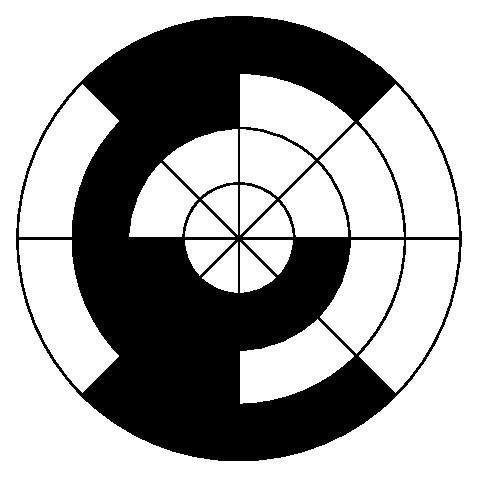
\includegraphics[scale=1]{images/encoderDiscAbsolute.eps}
\captionof{figure}{Poglądowy schemat dysku enkodera absolutnego z 3-bitowym kodem Graya\cite{bib:tarczaenkoderaabsolutnego}}
\label{fig:encoderDiscAbsolute}
\end{center}

Enkodery inkrementalne u~podstaw działają~w ten sam sposób, tzn. opierają się na dyskach kodujących, z~tą różnicą, że nie są w~stanie podać dokładnej wartości położenia. Zamiast tego, podają na wyjściu odpowiedni impuls przy obrocie w~danym kierunku. Następnie w~oprogramowaniu impulsy te są zliczane w celu oszacowania aktualnej pozycji względem pozycji startowej. Ze względu na wyzerowanie liczby impulsów przy utracie zasilania, ten typ enkodera nie jest w~stanie podać dokładnej pozycji w~przypadku utraty zasilania.

Istotny jest również podział enkoderów ze względu na wykorzystywane zjawisko fizyczne. Dwa główne typy to enkodery optyczne oraz magnetyczne. Oba rodzaje występują zarówno w~wariancie pojedynczym (Rysunek~\ref{fig:encoderDiscIncrementalSingle}) jak i~podwójnym (Rysunek~\ref{fig:encoderDiscIncrementalDual}). W~przypadku enkoderów optycznych, kolorowi białemu odpowiada szczelina, zaś kolorowi czarnemu blokada. W~przypadku enkoderów magnetycznych, kolorom odopowiadają bieguny~S~i~N.

\begin{figure}
    \centering
    \subfloat[Enkoder pojedynczy]{
      
\includegraphics[width=5cm]{images/encoderDiscIncrementalSingle.eps}
      \label{fig:encoderDiscIncrementalSingle}
    }\qquad
    \subfloat[Enkoder podwójny (kwadratowy)]{
      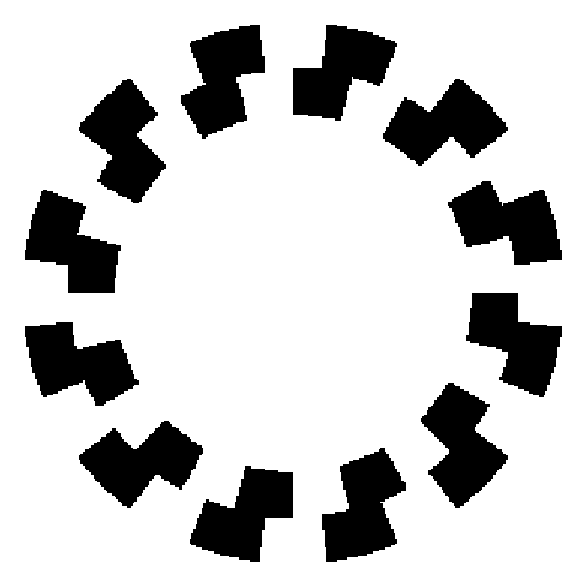
\includegraphics[width=5cm]{images/encoderDiscIncrementalDual.eps}
      \label{fig:encoderDiscIncrementalDual}
    }
    \caption{Poglądowe schematy dysku enkodera inkrementalnego \cite{bib:tarczeenkoderowinkrementalnych}}
\end{figure}

Jako że w~projekcie wykorzystane zostały enkodery magnetyczne, zasada ich działania została opisana, zaś enkodery optyczne pominięto. W enkoderze magnetycznym umieszcza się magnesy na obracającej się lub przemieszczającej się części obiektu~---~czyli dysku~---~a~czujniki magnetyczne~---~najczęściej czujniki Halla (Definicja~\ref{def:czujnikhalla})~---~znajdujące się na stałej części enkodera rejestrują zmiany pola magnetycznego (Rysunek~\ref{fig:obrazekenkoderamagnetycznego}). 

\begin{center}
  \includegraphics[scale=0.08]{images/magneticEncoder.png}
  \captionof{figure}{Zobrazowanie zasady działania enkodera magnetycznego dla tarczy z jednym rzędem\cite{bib:obrazekenkoderamagnetycznego}}
  \label{fig:obrazekenkoderamagnetycznego}
\end{center}

\begin{Definition}[Czujnik Halla]\label{def:czujnikhalla}
  Czujnik pola magnetycznego i~prądu, wykorzystujący zjawisko Halla.
\end{Definition}

Te zmiany są następnie przetwarzane na sygnały elektryczne, które można interpretować jako informacje o~kącie obrotu lub przemieszczeniu. Enkodery magnetyczne charakteryzują się wysoką dokładnością pomiaru, odpornością na wibracje i~brakiem kontaktu mechanicznego, dzięki czemu są odporne na zabrudzenia i~czynniki zewnętrzne takie jak kurz. Nie ma więc potrzeby osadzania ich w~zamkniętej przestrzeni, jak to ma miejsce z~czujnikami optycznymi.

\section{Regulacja sygnału sterującego}
\label{ch:regulatory}
Oprócz urządzenia (czujnika) dostarczającego sygnał informujący o fizycznym położeniu lub przemieszczeniu wału silnika, konieczne jest również zastosowanie metody wyznaczenia sygnału sterującego $u$. 

Trudno jest określić datę powstania pierwszych regulatorów. Pierwotnie nie były one tworzone z~myślą o~wyznaczaniu sygnału sterującego, lecz zwyczajnie jako część urządzeń. Przykładem jednego z~pierwszych regulatorów może być maszyna Ktesibiosa ---~wynaleziona w~III wieku~p.n.e.\cite{bib:regulatorktesibiusa} ---~w której rolę regulatora pełnił pływak dławiący wypływającą ze źródła wodę (Rysunek~\ref{fig:ktesibius}). Jest to prawdopodobnie pierwszy na świecie przykład regulatora proporcjonalnego.

\begin{center}
  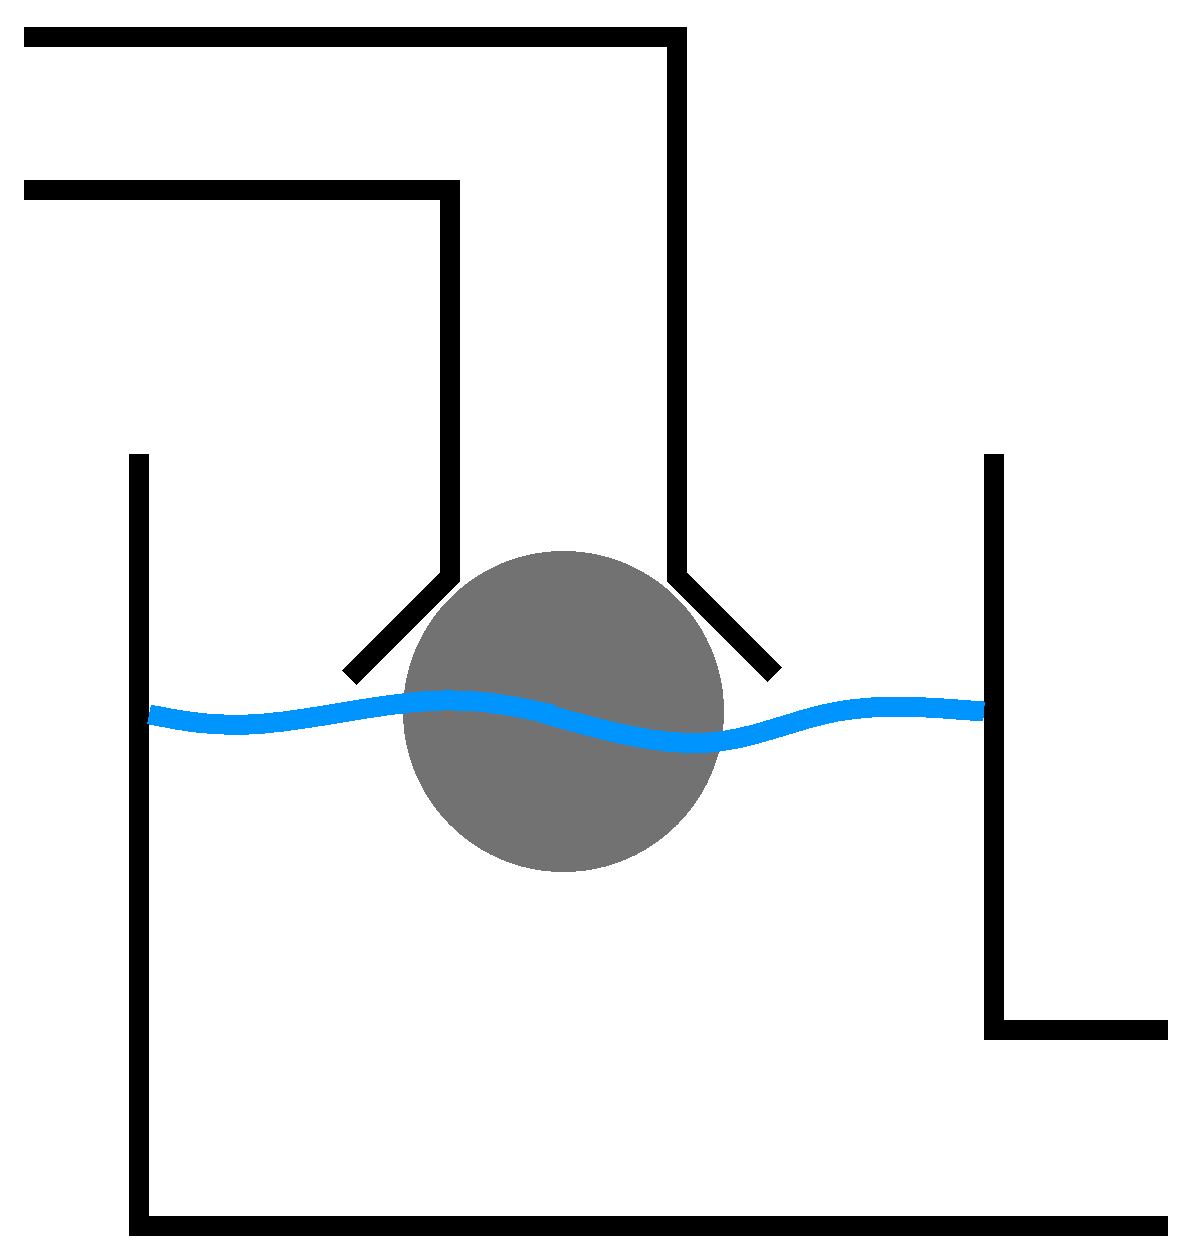
\includegraphics[scale=0.15]{images/ktesibius.png}
  \captionof{figure}{Zobrazowanie zasady działania regulatora Ktesibiosa}
  \label{fig:ktesibius}
\end{center}

Na przestrzeni kolejnych tysięcy lat w~technologii regulatorów nie dokonał się w~zasadzie żaden znaczący postęp. Dopiero w~XIX~i~XX~wieku rozpoczęły się badania nad teorią sterowania, w~których udział miało wielu naukowców z~całego świata. Lata prac doprowadziły do formalnego opracowania w~roku 1922 regulatora PID (ang.~\english{Proportional–Integral–Derivative}) (Definicja~\ref{def:pid}) przez rosyjskiego naukowca, Nicolasa Minorsky'ego\cite{bib:pidminorsky}.

\begin{Definition}[Regulator PID (Proporcjonalno-Integrująco-Różniczkujący)]\label{def:pid}
  Rrodzaj regulatora, który składa się z trzech elementów: proporcjonalnego (P), który reaguje na bieżącą wartość błędu (Definicja~ \ref{def:blad}) proporcjonalnie do niego; całkującego (I), który integruje bieżący błąd w czasie i reaguje na jego sumę; oraz różniczkującego (D), które reaguje na szybkość zmiany błędu. 
\end{Definition}

\begin{Definition}[Błąd; uchyb]\label{def:blad}
  W układach automatyki jest to różnica między wartością zadaną a zmierzoną wartością rzeczywistą.
\end{Definition}

Jego popularyzacja nastąpiła w~latach~'50~XX~wieku, gdy układy elektroniczne stały się tańsze, dotępniejsze i~bardziej niezawodne. Dziś jest powszechnie stosowany~w automatyce, robotyce, elektronice i~wielu innych dziedzinach inżynierii. Regulator PID jest stosowany najczęściej ze względu na prostotę, bardzo niski koszt implementacji i~wystarczające działanie w~większości przypadków.

Drugim najczęściej stosowanym regulatorem jest regulator predykcyjny MPC (ang.~\english{Model Predictive Control}). W~przeciwieństwie do tradycyjnych regulatorów które reagują na sprzężenie zwrotne z~wyjścia układu, regulator predykcyjny działa z~wyprzedzeniem, zanim zdąży nastąpić zmiana na wyjściu układu. 

Pierwsze wzmianki o~tym typie kontroli datowane są na wczesne lata '60~XX~wieku i~rozważania Rudolfa~E.~Kálmána na temat systemów liniowych. Od tego czasu, technologia regulatora predykcyjnego była rozwijana niezależnie przez wiele osób i~instytucji. W późnych latach '70~XX~wieku regulator ten można było już spotkać w ~zastosowaniach przemysłowych. W~roku 1979 zaprezentowano generację pierwszą, zaś najnowszą, 4~generację stanowią w~roku 1998\cite{bib:regulatormpc}. Pełna genealogia algorytmów MPC przedstawiona została na Rysunku~\ref{fig:regulatormpc}.

\begin{center}
  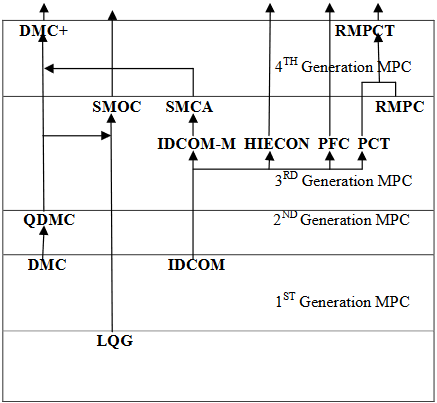
\includegraphics[scale=1]{images/drzewompc.png}
  \captionof{figure}{Genealogia algorytmów MPC\cite{bib:regulatormpc}}
  \label{fig:regulatormpc}
\end{center}

Regulatory predykcyjne znajdują zastosowanie w~układach o~dużym opóźnieniu i~wysokim rzędzie, gdzie regulatory PID są niewystarczające. Przykładem są sondy kosmiczne.

%%%%%%%%%%%%%% rozdział 3 - wymagania i narzędzia %%%%%%%%%%%%%%%%%
\chapter{Wymagania i narzędzia}
\label{ch:wymagania-i-narzedzia}

\begin{itemize}
\item wymagania funkcjonalne i niefunkcjonalne
\item przypadki użycia (diagramy UML) -- dla prac, w których mają zastosowanie
\item opis narzędzi, metod eksperymentalnych, metod modelowania itp.
\item metodyka pracy nad projektowaniem i implementacją -- dla prac, w których ma to zastosowanie
\end{itemize}

%%%%%%%%%%%%%% rozdział 4 - [Właściwy dla kierunku -- np. Specyfikacja zewnętrzna] %%%%%%%%%%%%%%%%%
\chapter{[Właściwy dla kierunku -- np. Specyfikacja zewnętrzna]}
\label{ch:04}

Jeśli „Specyfikacja zewnętrzna”:
\begin{itemize}
\item  wymagania sprzętowe i programowe
\item  sposób instalacji
\item  sposób aktywacji
\item  kategorie użytkowników
\item  sposób obsługi
\item  administracja systemem
\item  kwestie bezpieczeństwa
\item  przykład działania
\item  scenariusze korzystania z systemu (ilustrowane zrzutami z ekranu lub generowanymi dokumentami)
\end{itemize}

%%%%%%%%%%%%%%%%%%%%%
%% RYSUNEK Z PLIKU
%
%\begin{figure}
%\centering
%
\includegraphics[width=0.5\textwidth]{./politechnika_sl_logo_bw_pion_pl.pdf}
%\caption{Podpis rysunku zawsze pod rysunkiem.}
%\label{fig:etykieta-rysunku}
%\end{figure}
%Rys. \ref{fig:etykieta-rysunku} przestawia …
%%%%%%%%%%%%%%%%%%%%%
%
%%%%%%%%%%%%%%%%%%%%%
%% WIELE RYSUNKÓW 
%
%\begin{figure}
%\centering
%\begin{subfigure}{0.4\textwidth}
%    
\includegraphics[width=\textwidth]{./politechnika_sl_logo_bw_pion_pl.pdf}
%    \caption{Lewy górny rysunek.}
%    \label{fig:lewy-gorny}
%\end{subfigure}
%\hfill
%\begin{subfigure}{0.4\textwidth}
%    
\includegraphics[width=\textwidth]{./politechnika_sl_logo_bw_pion_pl.pdf}
%    \caption{Prawy górny rysunek.}
%    \label{fig:prawy-gorny}
%\end{subfigure}
%
%\begin{subfigure}{0.4\textwidth}
%    
\includegraphics[width=\textwidth]{./politechnika_sl_logo_bw_pion_pl.pdf}
%    \caption{Lewy dolny rysunek.}
%    \label{fig:lewy-dolny}
%\end{subfigure}
%\hfill
%\begin{subfigure}{0.4\textwidth}
%    
\includegraphics[width=\textwidth]{./politechnika_sl_logo_bw_pion_pl.pdf}
%    \caption{Prawy dolny rysunek.}
%    \label{fig:prawy-dolny}
%\end{subfigure}
%        
%\caption{Wspólny podpis kilku rysunków.}
%\label{fig:wiele-rysunkow}
%\end{figure}
%Rys. \ref{fig:wiele-rysunkow} przestawia wiele ważnych informacji, np. rys. \ref{fig:prawy-gorny} jest na prawo u góry.
%%%%%%%%%%%%%%%%%%%%%


 
\begin{figure}
\centering
\begin{tikzpicture}
\begin{axis}[
    y tick label style={
        /pgf/number format/.cd,
            fixed,   % po zakomentowaniu os rzednych jest indeksowana wykladniczo
            fixed zerofill, % 1.0 zamiast 1
            precision=1,
        /tikz/.cd
    },
    x tick label style={
        /pgf/number format/.cd,
            fixed,
            fixed zerofill,
            precision=2,
        /tikz/.cd
    }
]
\addplot [domain=0.0:0.1] {rnd};
\end{axis} 
\end{tikzpicture}
\caption{Podpis rysunku po rysunkiem.}
\label{fig:2}
\end{figure}


%%%%%%%%%%%%%% rozdział 5 - [Właściwy dla kierunku -- np. Specyfikacja wewnętrzna] %%%%%%%%%%%%%%%%%
\chapter{[Właściwy dla kierunku -- np. Specyfikacja wewnętrzna]}
\label{ch:05}


Jeśli „Specyfikacja wewnętrzna”:
\begin{itemize}
\item przedstawienie idei
\item architektura systemu
\item opis struktur danych (i organizacji baz danych)
\item komponenty, moduły, biblioteki, przegląd ważniejszych klas (jeśli występują)
\item przegląd ważniejszych algorytmów (jeśli występują)
\item szczegóły implementacji wybranych fragmentów, zastosowane wzorce projektowe
\item diagramy UML
\end{itemize}

% % % % % % % % % % % % % % % % % % % % % % % % % % % % % % % % % % % 
% Pakiet minted wymaga importu: \usepackage{minted}                 %
% i specjalnego kompilowania:                                       %
% pdflatex -shell-escape main                                       %
% % % % % % % % % % % % % % % % % % % % % % % % % % % % % % % % % % % 


Krótka wstawka kodu w linii tekstu jest możliwa, np.  \lstinline|int a;| (biblioteka \texttt{listings})% lub  \mintinline{C++}|int a;| (biblioteka \texttt{minted})
. 
Dłuższe fragmenty lepiej jest umieszczać jako rysunek, np. kod na rys \ref{fig:pseudokod:listings}% i rys. \ref{fig:pseudokod:minted}
, a naprawdę długie fragmenty – w załączniku.


\begin{figure}
\centering
\begin{lstlisting}
class test : public basic
{
    public:
      test (int a);
      friend std::ostream operator<<(std::ostream & s, 
                                     const test & t);
    protected:
      int _a;  
      
};
\end{lstlisting}
\caption{Pseudokod w \texttt{listings}.}
\label{fig:pseudokod:listings}
\end{figure}

%\begin{figure}
%\centering
%\begin{minted}[linenos,frame=lines]{c++}
%class test : public basic
%{
%    public:
%      test (int a);
%      friend std::ostream operator<<(std::ostream & s, 
%                                     const test & t);
%    protected:
%      int _a;  
%      
%};
%\end{minted}
%\caption{Pseudokod w \texttt{minted}.}
%\label{fig:pseudokod:minted}
%\end{figure}

%%%%%%%%%%%%%% rozdział 6 - Weryfikacja i walidacja %%%%%%%%%%%%%%%%%
\chapter{Weryfikacja i walidacja}
\label{ch:06}
\begin{itemize}
\item sposób testowania w ramach pracy (np. odniesienie do modelu V)
\item organizacja eksperymentów
\item przypadki testowe zakres testowania (pełny/niepełny)
\item wykryte i usunięte błędy
\item opcjonalnie wyniki badań eksperymentalnych
\end{itemize}

\begin{table}
\centering
\caption{Nagłówek tabeli jest nad tabelą.}
\label{id:tab:wyniki}
\begin{tabular}{rrrrrrrr}
\toprule
	         &                                     \multicolumn{7}{c}{metoda}                                      \\
	         \cmidrule{2-8}
	         &         &         &        \multicolumn{3}{c}{alg. 3}        & \multicolumn{2}{c}{alg. 4, $\gamma = 2$} \\
	         \cmidrule(r){4-6}\cmidrule(r){7-8}
	$\zeta$ &     alg. 1 &   alg. 2 & $\alpha= 1.5$ & $\alpha= 2$ & $\alpha= 3$ &   $\beta = 0.1$  &   $\beta = -0.1$ \\
\midrule
	       0 &  8.3250 & 1.45305 &       7.5791 &    14.8517 &    20.0028 & 1.16396 &                       1.1365 \\
	       5 &  0.6111 & 2.27126 &       6.9952 &    13.8560 &    18.6064 & 1.18659 &                       1.1630 \\
	      10 & 11.6126 & 2.69218 &       6.2520 &    12.5202 &    16.8278 & 1.23180 &                       1.2045 \\
	      15 &  0.5665 & 2.95046 &       5.7753 &    11.4588 &    15.4837 & 1.25131 &                       1.2614 \\
	      20 & 15.8728 & 3.07225 &       5.3071 &    10.3935 &    13.8738 & 1.25307 &                       1.2217 \\
	      25 &  0.9791 & 3.19034 &       5.4575 &     9.9533 &    13.0721 & 1.27104 &                       1.2640 \\
	      30 &  2.0228 & 3.27474 &       5.7461 &     9.7164 &    12.2637 & 1.33404 &                       1.3209 \\
	      35 & 13.4210 & 3.36086 &       6.6735 &    10.0442 &    12.0270 & 1.35385 &                       1.3059 \\
	      40 & 13.2226 & 3.36420 &       7.7248 &    10.4495 &    12.0379 & 1.34919 &                       1.2768 \\
	      45 & 12.8445 & 3.47436 &       8.5539 &    10.8552 &    12.2773 & 1.42303 &                       1.4362 \\
	      50 & 12.9245 & 3.58228 &       9.2702 &    11.2183 &    12.3990 & 1.40922 &                       1.3724 \\
\bottomrule
\end{tabular}
\end{table}  

%%%%%%%%%%%%%% rozdział 7 - Podsumowanie i wnioski %%%%%%%%%%%%%%%%%
\chapter{Podsumowanie i wnioski}
\begin{itemize}
    \item uzyskane wyniki w świetle postawionych celów i zdefiniowanych wyżej wymagań
    \item kierunki ewentualnych danych prac (rozbudowa funkcjonalna …)
    \item problemy napotkane w trakcie pracy
    \end{itemize}
    
    
    
    \backmatter
    
    %\bibliographystyle{plplain}  % bibtex
    %\bibliography{biblio} % bibtex
    \printbibliography           % biblatex
    \addcontentsline{toc}{chapter}{Bibliografia}
    
    \begin{appendices}


\backmatter
%\bibliographystyle{plplain}  % bibtex
%\bibliography{biblio} % bibtex
\printbibliography           % biblatex
\addcontentsline{toc}{chapter}{Bibliografia}

\begin{appendices}

%%%%%%%%%%%%%% rozdział 8 - Spis skrótów i symboli %%%%%%%%%%%%%%%%%
\chapter{Spis skrótów i symboli}
\begin{itemize}
\item[$u$] sygnał sterujący obiektem wykonawczym w układzie sterowania/regulacji
\item[PID] regulator Proporcjonalno-Całkująco-Różniczkujący (ang.~\english{Proportional–Integral–Derivative})
\item[MPC] regulator oparty na modelu predykcyjnym (ang.~\english{Model Predictive Control})
\end{itemize}

%%%%%%%%%%%%%% rozdział 9 - Źródła %%%%%%%%%%%%%%%%%
\chapter{Źródła}
Jeżeli w pracy konieczne jest umieszczenie długich fragmentów kodu źródłowego, należy je przenieść w to miejsce.

\begin{lstlisting}
if (_nClusters < 1)
	throw std::string ("unknown number of clusters");
if (_nIterations < 1 and _epsilon < 0)
	throw std::string ("You should set a maximal number of iteration or minimal difference -- epsilon.");
if (_nIterations > 0 and _epsilon > 0)
	throw std::string ("Both number of iterations and minimal epsilon set -- you should set either number of iterations or minimal epsilon.");
\end{lstlisting}


% % % % % % % % % % % % % % % % % % % % % % % % % % % % % % % % % % % 
% Pakiet minted wymaga odkomentowania w pliku config/settings.tex   %
% importu pakietu minted: \usepackage{minted}                       %
% i specjalnego kompilowania:                                       %
% pdflatex -shell-escape praca                                      %
% % % % % % % % % % % % % % % % % % % % % % % % % % % % % % % % % % % 

%\begin{minted}[linenos,breaklines,frame=lines]{c++}
%if (_nClusters < 1)
%   throw std::string ("unknown number of clusters");
%if (_nIterations < 1 and _epsilon < 0)
%   throw std::string ("You should set a maximal number of iteration or minimal difference -- epsilon.");
%if (_nIterations > 0 and _epsilon > 0)
%   throw std::string ("Both number of iterations and minimal epsilon set -- you should set either number of iterations or minimal epsilon.");
%\end{minted}

%%%%%%%%%%%%%% rozdział 10 - Lista dodatkowych plików, uzupełniających tekst pracy %%%%%%%%%%%%%%%%%
\chapter{Lista dodatkowych plików, uzupełniających tekst pracy} 
W systemie do pracy dołączono dodatkowe pliki zawierające:
\begin{itemize}
\item źródła programu,
\item dane testowe,
\item film pokazujący działanie opracowanego oprogramowania lub zaprojektowanego i~wykonanego urządzenia,
\item itp.
\end{itemize}

\end{appendices}
\end{document}


%% Finis coronat opus.